% \begin{figure}[H]
%     \centering
%     \includegraphics[width=0.8\linewidth]{billeder/Danish inflation seasonal subseries.png}
%     \\[\smallskipamount]
%     \includegraphics[width=0.8\linewidth]{billeder/Danish unemployment seasonal subseries.png}
%     \\[\smallskipamount]
%     \includegraphics[width=0.8\linewidth]{billeder/Ez inflation seasonal subseries.png}
%     \\[\smallskipamount]
%     \includegraphics[width=0.8\linewidth]{billeder/EZ unemployment seasonal subseries.png}
%     \caption{Caption}
%     \label{fig: All seasonal subseries plots}
% \end{figure}







\appendix
\chapter{Appendix}
\section{Data}


\subsection{Seasonality with sub-seriesplots}
\begin{figure}[H]
    \centering
    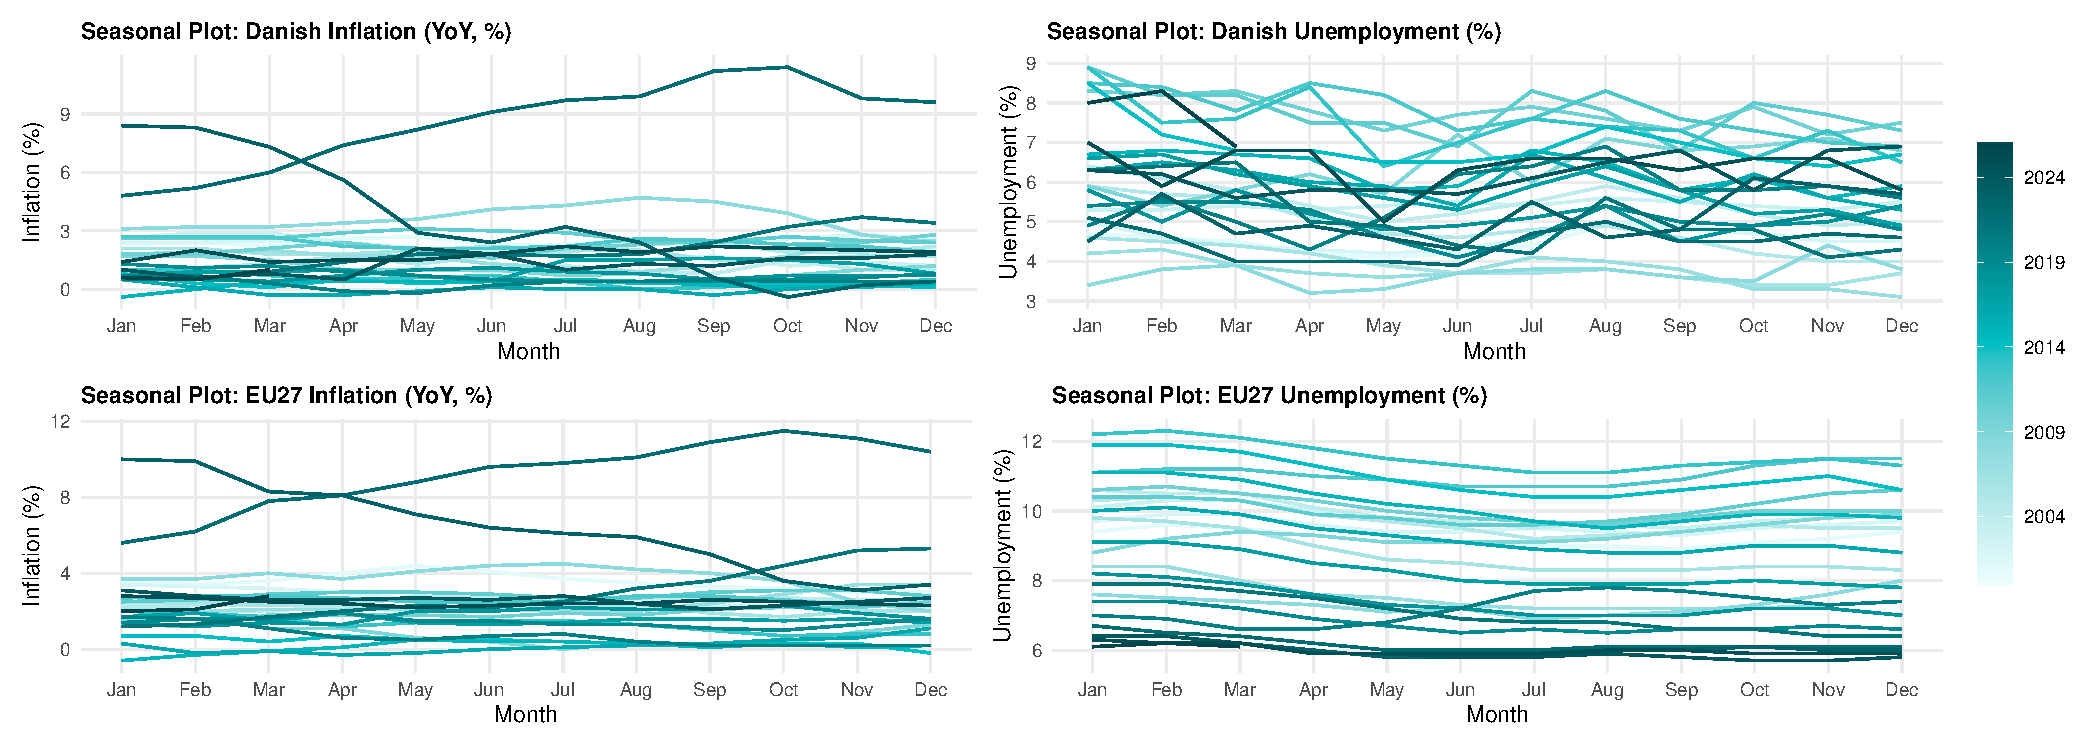
\includegraphics[width=1\linewidth]{billeder/subseason.pdf}
    \caption{Unemployment shows some seasonal behavior, especially in the euro area, while HICP shows little clear seasonality in this plot.}
    \label{fig:index_seasonal_plot}
\end{figure}

\begin{figure}[H]
    \centering
    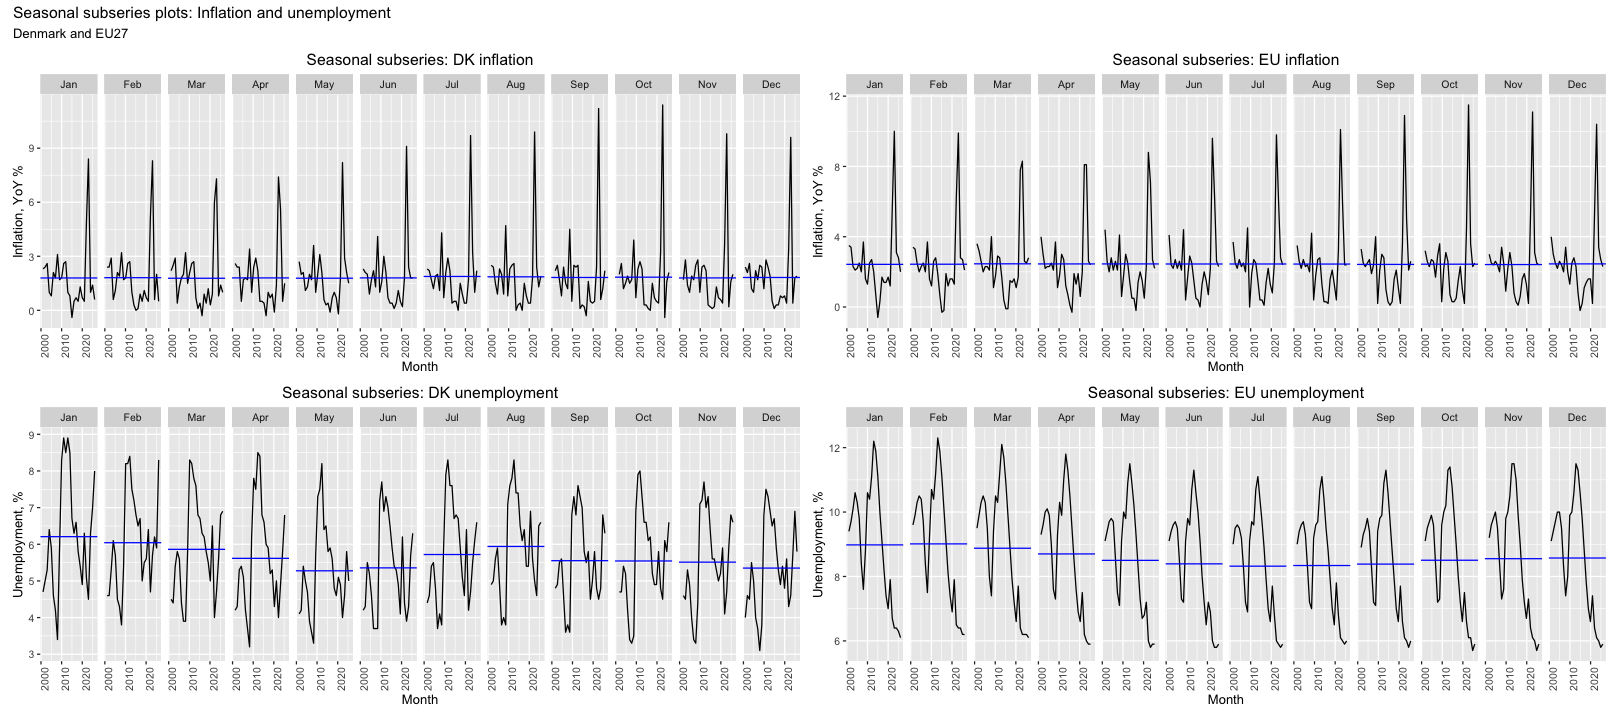
\includegraphics[width=1\linewidth]{Bilag/subseries-plot.png}
    \caption{We see the clear no seasonality of inflation, and the slight seasonality of unemployment, but particularly the EU unemployment}
    \label{fig:subseries-plot}
\end{figure}





\subsection{Making data stationary}\label{sec:appendix_acf_pacf}

% --- Danish inflation (stationary in levels) ---
\begin{figure}[H]
    \centering
    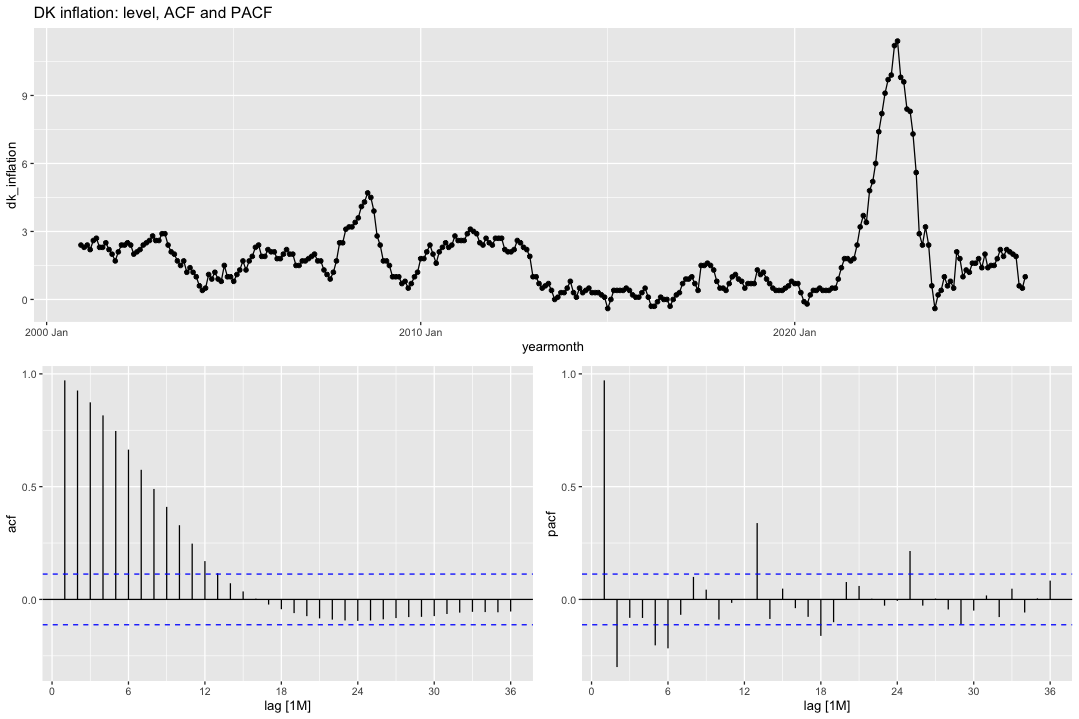
\includegraphics[width=0.7\linewidth]{billeder/dk_inflation_acf_pacf.png}
    \caption{Time series, ACF and PACF for Danish inflation in levels.}
    \label{fig:dk_inflation_acf_pacf}
\end{figure}

% --- Danish unemployment: levels vs. first difference ---
\begin{figure}[H]
    \centering
    \begin{subfigure}{0.49\linewidth}
        \centering
        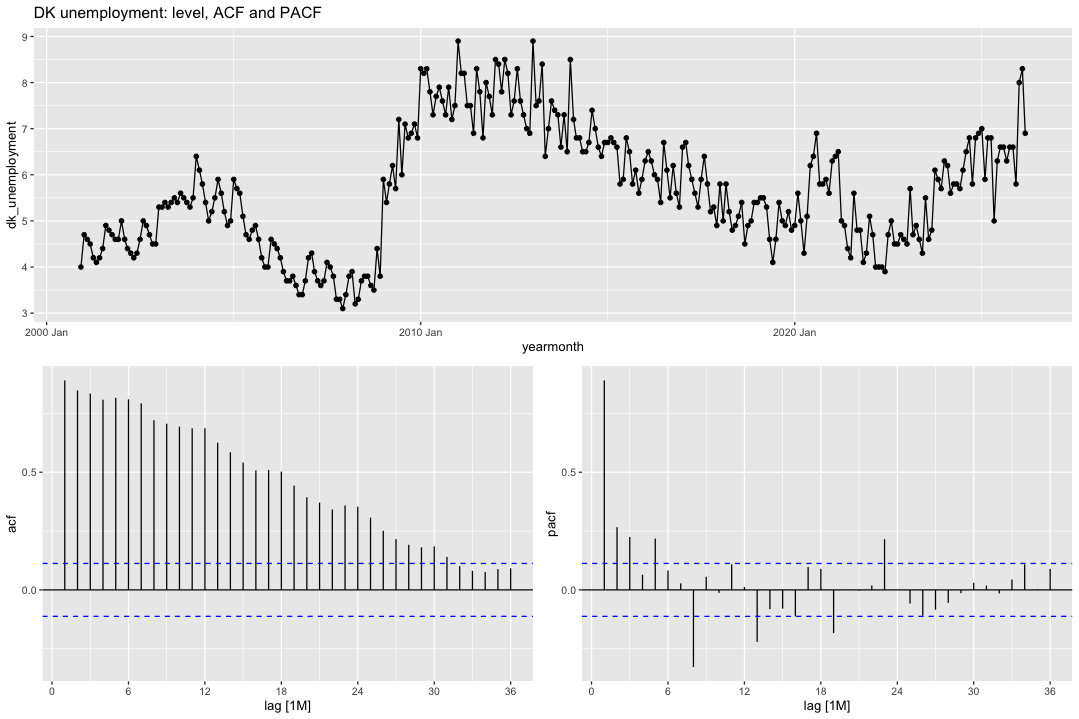
\includegraphics[width=\linewidth]{billeder/dk_unemployment_acf_pacf.png}
        \caption{Levels.}
        \label{fig:dk_unemployment_acf_pacf}
    \end{subfigure}
    \hfill
    \begin{subfigure}{0.49\linewidth}
        \centering
        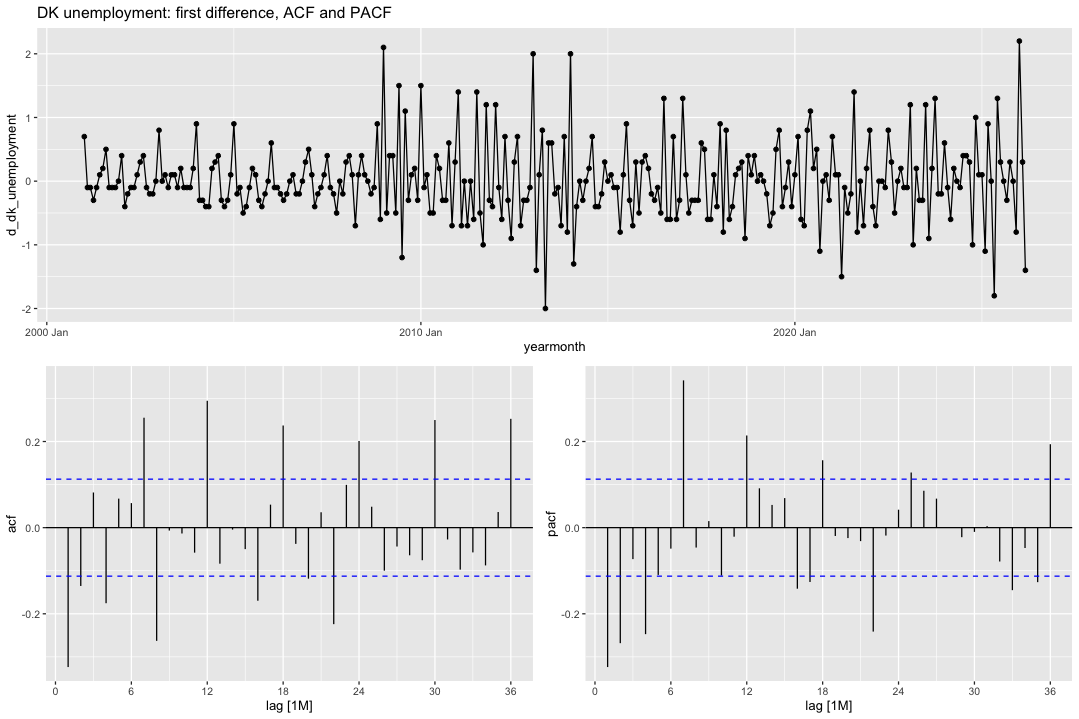
\includegraphics[width=\linewidth]{billeder/dk_diff_unemployment_acf_pacf.png}
        \caption{First-differenced.}
        \label{fig:dk_diff_unemployment_acf_pacf}
    \end{subfigure}
    \caption{Time series, ACF and PACF for Danish unemployment.}
    \label{fig:dk_unemployment_combined}
\end{figure}

% --- EU27 inflation: levels vs. first difference ---
\begin{figure}[H]
    \centering
    \begin{subfigure}{0.49\linewidth}
        \centering
        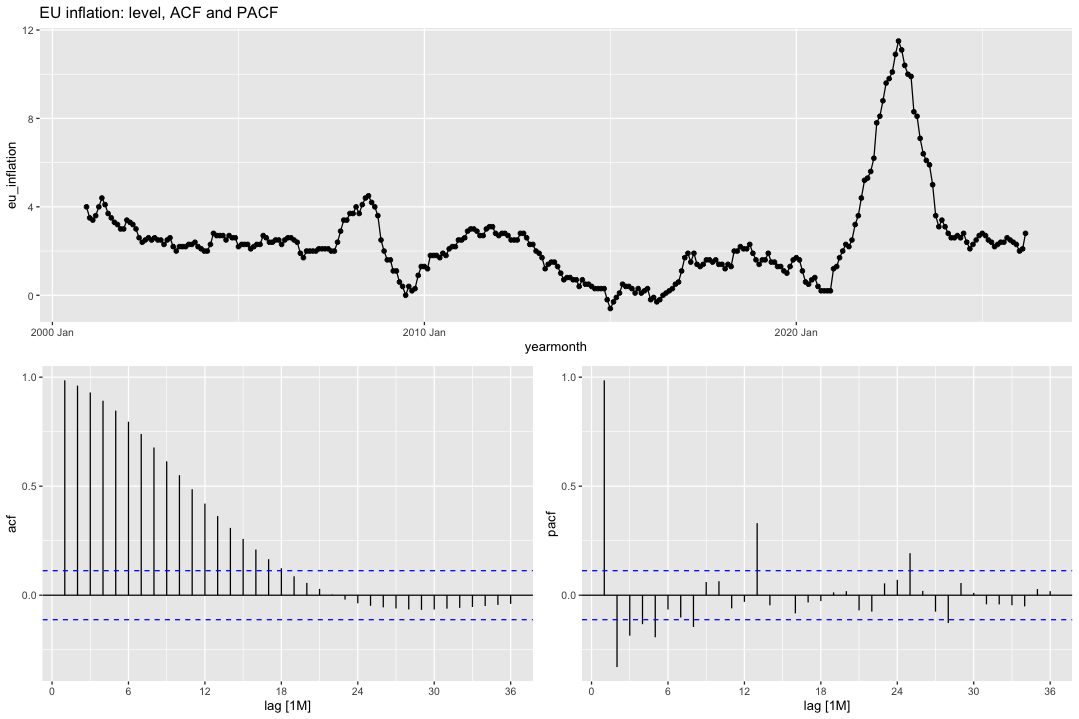
\includegraphics[width=\linewidth]{billeder/eu_inflation_acf_pacf.png}
        \caption{Levels.}
        \label{fig:eu_inflation_acf_pacf}
    \end{subfigure}
    \hfill
    \begin{subfigure}{0.49\linewidth}
        \centering
        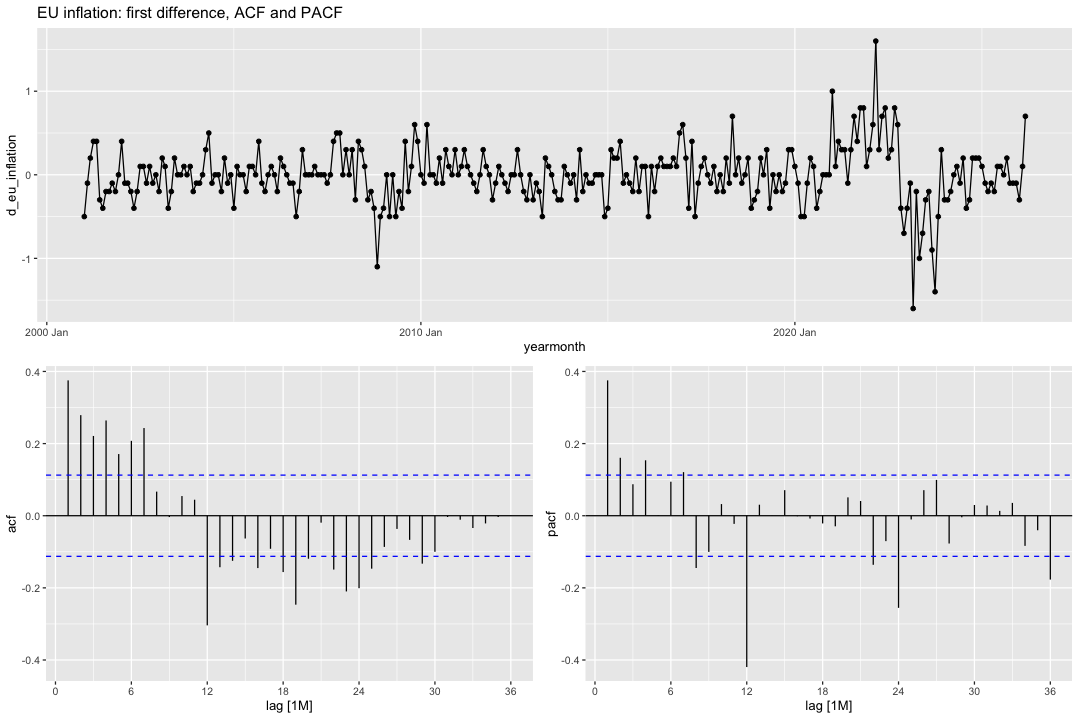
\includegraphics[width=\linewidth]{billeder/eu_diff_inflation_acf_pacf.png}
        \caption{First-differenced.}
        \label{fig:eu_diff_inflation_acf_pacf}
    \end{subfigure}
    \caption{Time series, ACF and PACF for EU27 inflation.}
    \label{fig:eu_inflation_combined}
\end{figure}

% --- EU27 unemployment: levels vs. first difference ---
\begin{figure}[H]
    \centering
    \begin{subfigure}{0.49\linewidth}
        \centering
        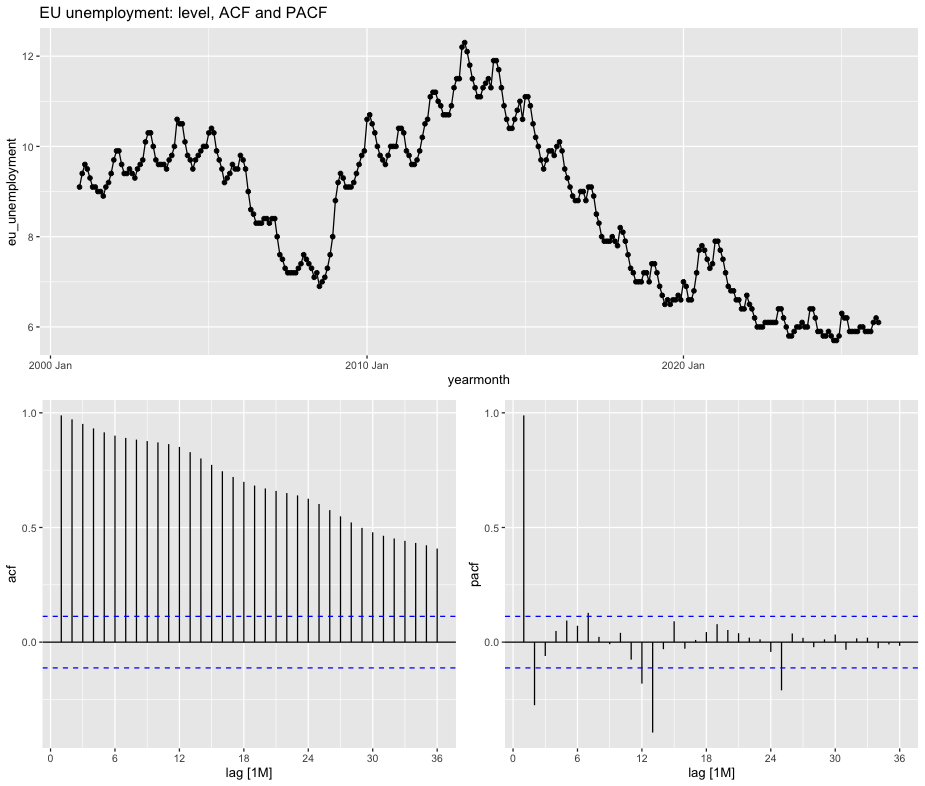
\includegraphics[width=\linewidth]{billeder/eu_unemployment_acf_pacf.png}
        \caption{Levels.}
        \label{fig:eu_unemployment_acf_pacf}
    \end{subfigure}
    \hfill
    \begin{subfigure}{0.49\linewidth}
        \centering
        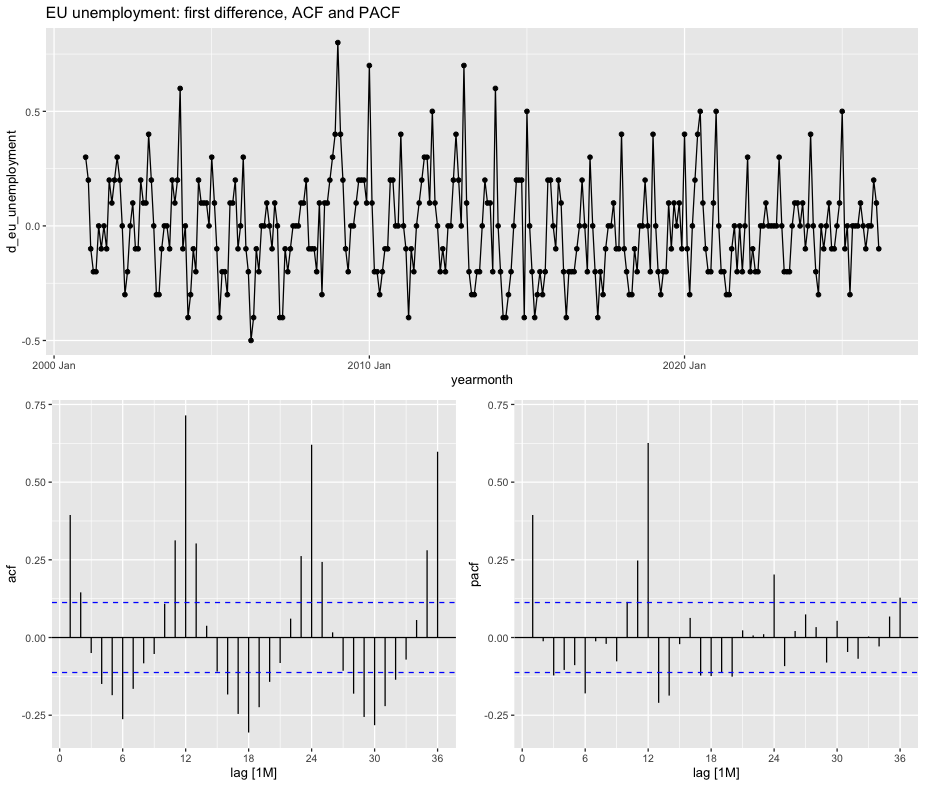
\includegraphics[width=\linewidth]{billeder/eu_diff_unemployment_acf_pacf.png}
        \caption{First-differenced.}
        \label{fig:eu_diff_unemployment_acf_pacf}
    \end{subfigure}
    \caption{Time series, ACF and PACF for EU27 unemployment.}
    \label{fig:eu_unemployment_combined}
\end{figure}


\subsection{Model output}\label{sec:appendix_model_output}
% -------------------------------------------------------
\subsubsection{ARIMA - Naive}
% -------------------------------------------------------
\begin{figure}[H]
    \centering
    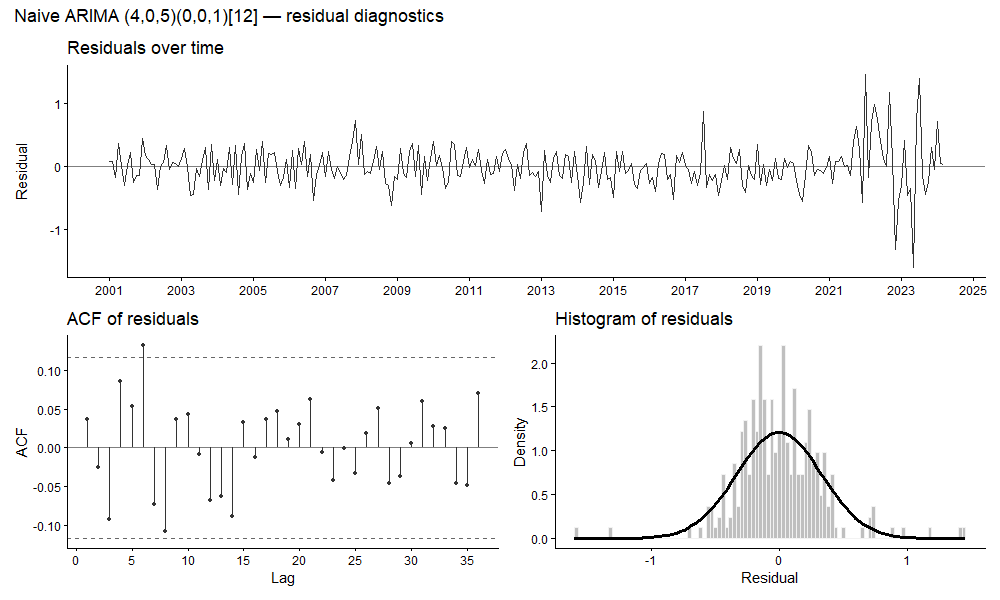
\includegraphics[width=0.8\linewidth]{billeder/Naiv_arima_diagnostics.png}
    \caption{Residuals from Naive ARIMA}
    \label{fig:placeholder}
\end{figure}


% -------------------------------------------------------
\subsubsection{ARIMA - Pre-Surge}
% -------------------------------------------------------
\begin{figure}[H]
    \centering
    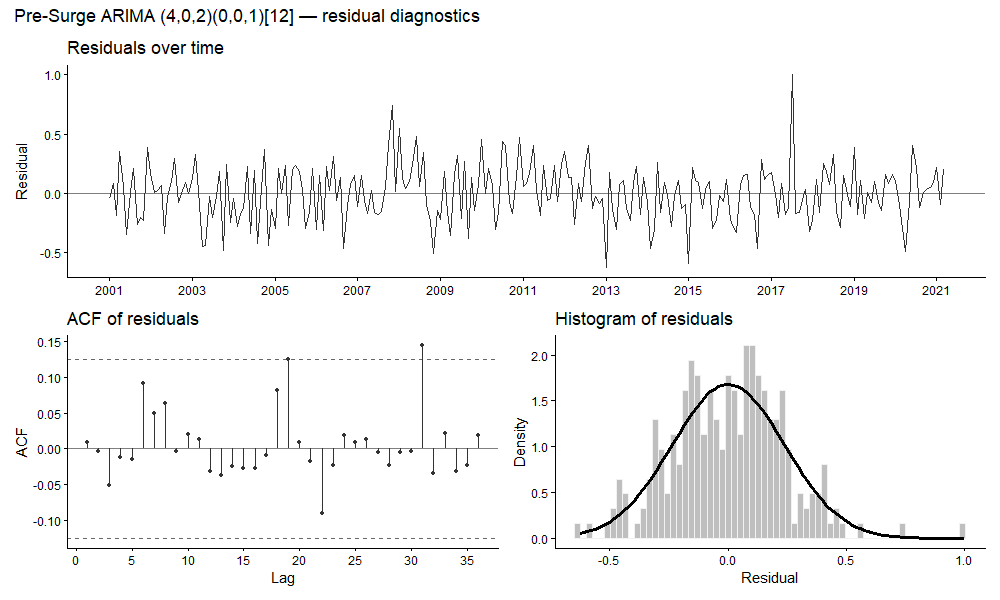
\includegraphics[width=0.8\linewidth]{billeder/Pre_surge_diagnostics.png}
    \caption{Residuals from Pre-Surge ARIMA}
    \label{fig:placeholder}
\end{figure}


% -------------------------------------------------------
\subsubsection{Dynamic Regression - Phillips Curve - Model}
% -------------------------------------------------------
\begin{figure}[H]
    \centering
    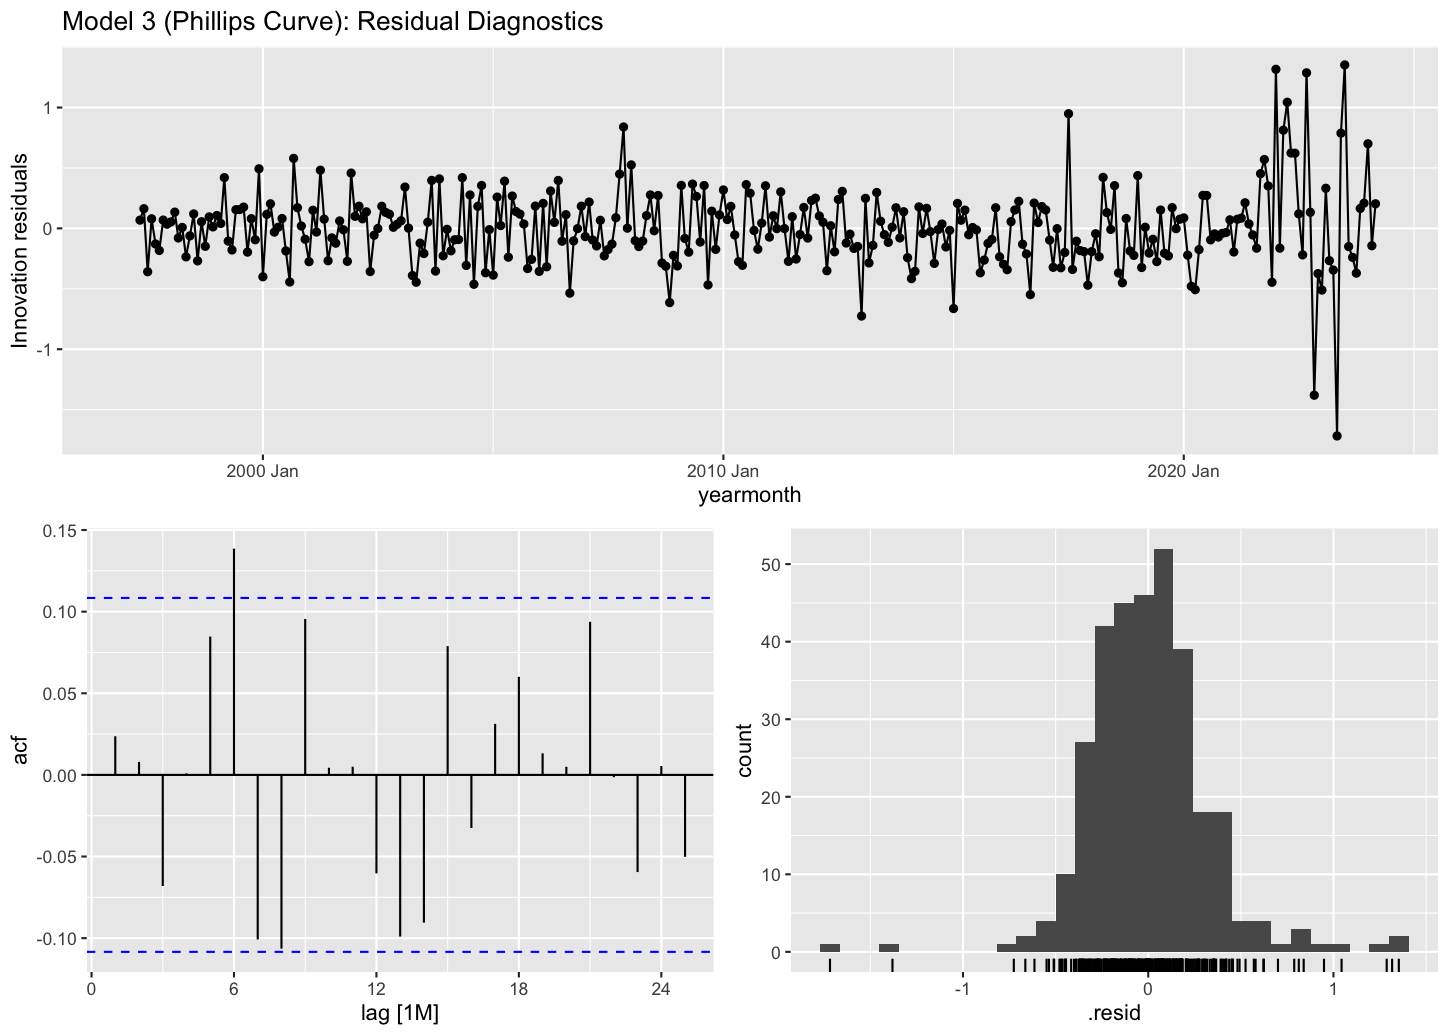
\includegraphics[width=0.8\linewidth]{billeder/Phillips_curve_model_residuals.png}
    \caption{Dynamic regression, Phillips curve, Residuals}
    \label{fig:phillips_curve_residuals}
\end{figure}

\begin{figure}[H]
    \centering
    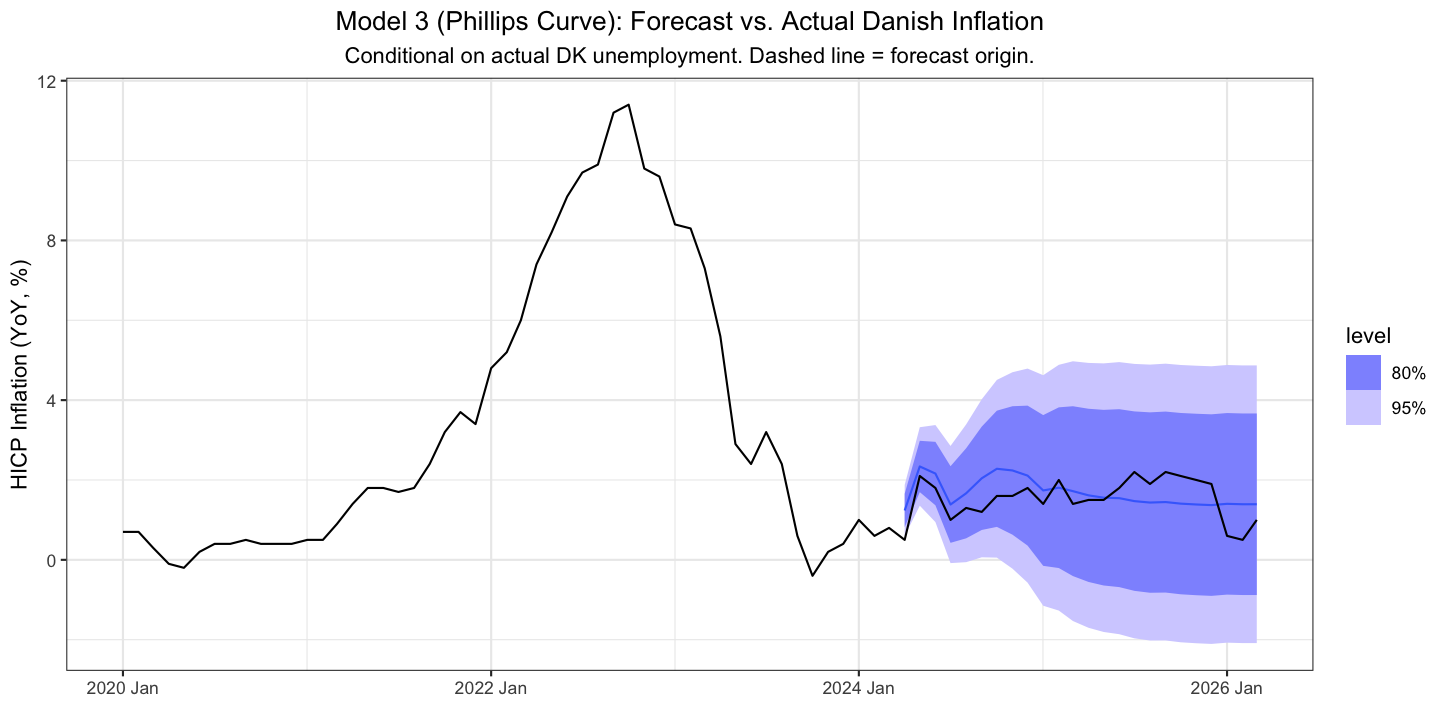
\includegraphics[width=0.8\linewidth]{billeder/Phillips_curve_model_forecast.png}
    \caption{Dynamic regression, Phillips curve out of sample model fit}
    \label{fig:phillips_curve_forecast}
\end{figure}


\begin{table}[H]
\centering
\caption{Model 3 (Phillips Curve) coefficient estimates with p-values}
\small{
\begin{tabular*}{\textwidth}{@{\extracolsep{\fill}}lcccc}
\hline \hline
\rule{0pt}{12pt}\textbf{Parameter} & \textbf{Estimate} & \textbf{Std. err} & \textbf{$t$-stat} & \textbf{$p$-value} \\[4pt]
\hline
\rule{0pt}{12pt}AR(1)        & $1.847$  & $(0.053)$ & $34.85$  & $<0.001$ \\[4pt]
AR(2)                        & $-0.855$ & $(0.052)$ & $-16.44$ & $<0.001$ \\[4pt]
MA(1)                        & $-0.675$ & $(0.073)$ & $-9.25$  & $<0.001$ \\[4pt]
MA(2)                        & $-0.182$ & $(0.062)$ & $-2.94$  & $0.003$  \\[4pt]
MA(3)                        & $0.214$  & $(0.064)$ & $3.34$   & $0.001$  \\[4pt]
SMA(1)                       & $-0.635$ & $(0.054)$ & $-11.76$ & $<0.001$ \\[4pt]
Intercept                    & $1.807$  & $(0.295)$ & $6.13$   & $<0.001$ \\[4pt]
\hline
\rule{0pt}{12pt}$\Delta u^{\text{DK}}_{t}$   & $-0.011$ & $(0.022)$ & $-0.50$ & $0.617$ \\[4pt]
$\Delta u^{\text{DK}}_{t-1}$                 & $-0.033$ & $(0.036)$ & $-0.92$ & $0.359$ \\[4pt]
$\Delta u^{\text{DK}}_{t-2}$                 & $-0.027$ & $(0.041)$ & $-0.66$ & $0.510$ \\[4pt]
$\Delta u^{\text{DK}}_{t-3}$                 & $-0.025$ & $(0.038)$ & $-0.66$ & $0.510$ \\[4pt]
$\Delta u^{\text{DK}}_{t-4}$                 & $-0.053$ & $(0.040)$ & $-1.33$ & $0.185$ \\[4pt]
$\Delta u^{\text{DK}}_{t-5}$                 & $-0.048$ & $(0.036)$ & $-1.33$ & $0.182$ \\[4pt]
$\Delta u^{\text{DK}}_{t-6}$                 & $-0.006$ & $(0.022)$ & $-0.27$ & $0.785$ \\[4pt]
\hline \hline
\multicolumn{5}{l}{\rule{0pt}{12pt}\footnotesize $\hat{\sigma}^2 = 0.105$,\;
AICc $= 221.6$,\; BIC $= 276.9$.}
\end{tabular*}
}
\label{tab:phillips_coef_appendix}
\end{table}


% -------------------------------------------------------
\subsubsection{GETS Model}
% -------------------------------------------------------


\begin{figure}[H]
    \centering
    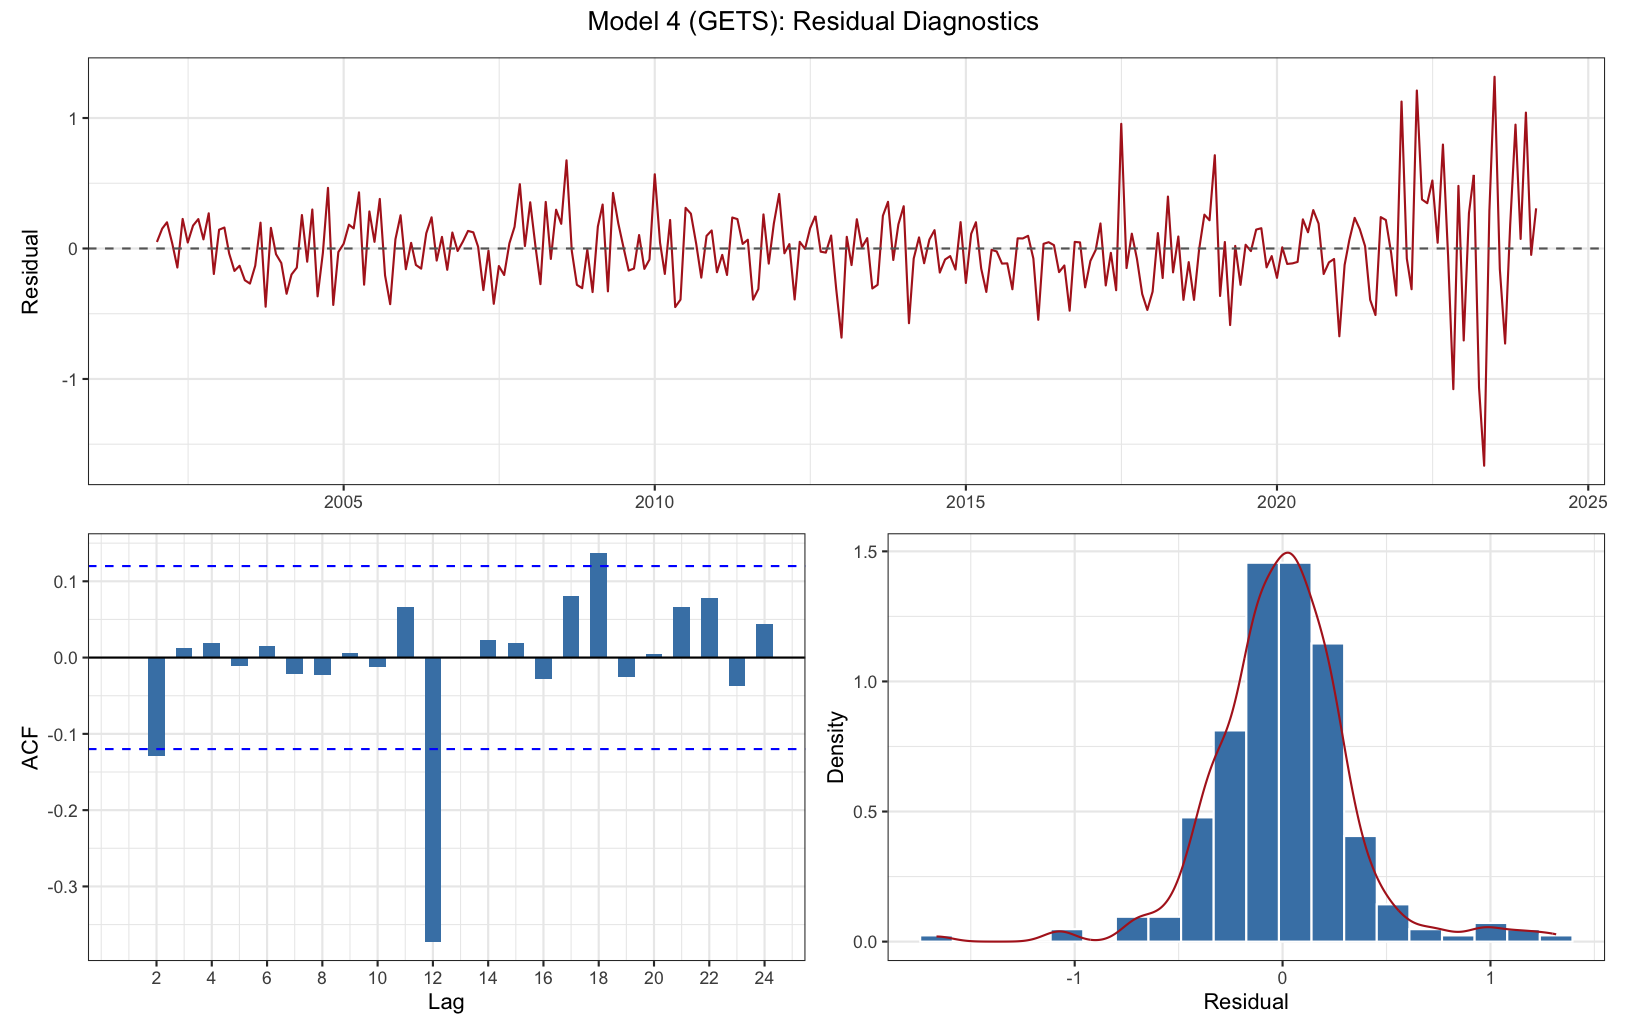
\includegraphics[width=0.8\linewidth]{billeder/GETS_residuals.png}
    \caption{GETS Residuals}
    \label{fig:gets_residuals}
\end{figure}

\begin{figure}[H]
    \centering
    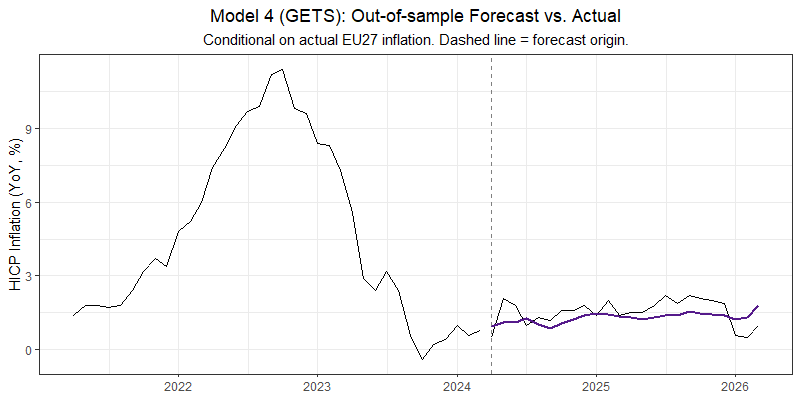
\includegraphics[width=0.8\linewidth]{billeder/Gets_plot.png}
    \caption{GETS out of sample model fit}
    \label{fig:gets_forecast}
\end{figure}


\begin{table}[H]
\centering
\caption{GUM mean equation estimates. Bold rows indicate variables retained in the
final GETS specification.}
\small{
\begin{tabular*}{\textwidth}{@{\extracolsep{\fill}}lcccc}
\hline \hline
\rule{0pt}{12pt}\textbf{Parameter} & \textbf{Estimate} & \textbf{Std. err} & \textbf{$t$-stat} & \textbf{$p$-value} \\[4pt]
\hline
\rule{0pt}{12pt}\textbf{Const}                 & $\mathbf{0.095}$ & $\mathbf{(0.032)}$ & $\mathbf{3.001}$ & $\mathbf{0.003^{**}}$ \\[2pt]
\textbf{AR(1)}                                  & $\mathbf{0.967}$ & $\mathbf{(0.065)}$ & $\mathbf{14.770}$ & $\mathbf{{<}0.001^{***}}$ \\[2pt]
AR(2)                                           & $-0.175$ & $(0.090)$ & $-1.942$ & $0.053^{\dagger}$ \\[2pt]
\textbf{AR(3)}                                  & $\mathbf{0.196}$ & $\mathbf{(0.094)}$ & $\mathbf{2.093}$ & $\mathbf{0.037^{*}}$ \\[2pt]
AR(4)                                           & $0.001$ & $(0.097)$ & $0.007$ & $0.995$ \\[2pt]
AR(5)                                           & $0.048$ & $(0.097)$ & $0.492$ & $0.623$ \\[2pt]
\textbf{AR(6)}                                  & $\mathbf{-0.098}$ & $\mathbf{(0.072)}$ & $\mathbf{-1.364}$ & $\mathbf{0.174}$ \\[2pt]
Surge dummy                                     & $0.108$ & $(0.102)$ & $1.056$ & $0.292$ \\[2pt]
$\Delta u_{t}$                                  & $0.062$ & $(0.041)$ & $1.496$ & $0.136$ \\[2pt]
$\Delta u_{t-1}$                                & $0.096$ & $(0.047)$ & $2.059$ & $0.041^{*}$ \\[2pt]
$\Delta u_{t-2}$                                & $0.077$ & $(0.049)$ & $1.564$ & $0.119$ \\[2pt]
$\Delta u_{t-3}$                                & $0.066$ & $(0.048)$ & $1.387$ & $0.167$ \\[2pt]
$\Delta u_{t-4}$                                & $0.039$ & $(0.049)$ & $0.786$ & $0.433$ \\[2pt]
$\Delta u_{t-5}$                                & $0.056$ & $(0.046)$ & $1.204$ & $0.230$ \\[2pt]
$\Delta u_{t-6}$                                & $0.053$ & $(0.041)$ & $1.281$ & $0.201$ \\[2pt]
$\pmb{\pi}^{\text{EZ}}_{t}$           & $\mathbf{0.670}$ & $\mathbf{(0.079)}$ & $\mathbf{8.502}$ & $\mathbf{{<}0.001^{***}}$ \\[2pt]
$\pi^{\text{EZ}}_{t-1}$                  & $0.154$ & $(0.089)$ & $1.723$ & $0.086^{\dagger}$ \\[2pt]
$\pi^{\text{EZ}}_{t-2}$                  & $0.185$ & $(0.089)$ & $2.069$ & $0.040^{*}$ \\[2pt]
$ \pi^{\text{EZ}}_{t-3}$                  & $0.068$ & $(0.091)$ & $0.744$ & $0.458$ \\[2pt]
$ \pi^{\text{EZ}}_{t-4}$                  & $-0.115$ & $(0.090)$ & $-1.279$ & $0.202$ \\[2pt]
$ \pi^{\text{EZ}}_{t-5}$                  & $0.116$ & $(0.088)$ & $1.320$ & $0.188$ \\[2pt]
$ \pi^{\text{EZ}}_{t-6}$                 & $0.025$ & $(0.076)$ & $0.324$ & $0.746$ \\[4pt]
\hline \hline
\multicolumn{5}{l}{\footnotesize $^{***}p<0.001$,\; $^{**}p<0.01$,\; $^{*}p<0.05$,\; $^{\dagger}p<0.10$}
\end{tabular*}
}
\label{tab:gum_coef}
\end{table}